\documentclass[10pt]{article}
\usepackage[a4paper, margin=2cm]{geometry}
\usepackage[utf8]{inputenc}
\usepackage{graphicx}
\usepackage{lastpage}
\usepackage{fancyhdr}

\pagestyle{fancy}
\fancyhf{}
\rfoot{Page \thepage \hspace{1pt} sur \pageref{LastPage}}

\begin{document}

\title{\textbf{Math - Devoir Formatif}}
\author{Hovinne Noé}
\date{}
\maketitle

\section*{Exercice 30 (p. 154) : calculer le volume d'un solide}\vspace{0.2cm}

%----------------------------------------------------------------------------------------------------------------------------------------
\flushleft \textbf{a.1) Établir la formule permettant de calculer le volume d'un cylindre droit de rayon \textit{R} et de hauteur \textit{h}}
\begin{figure}[h]
    \textit{\caption{}}
    \centering
    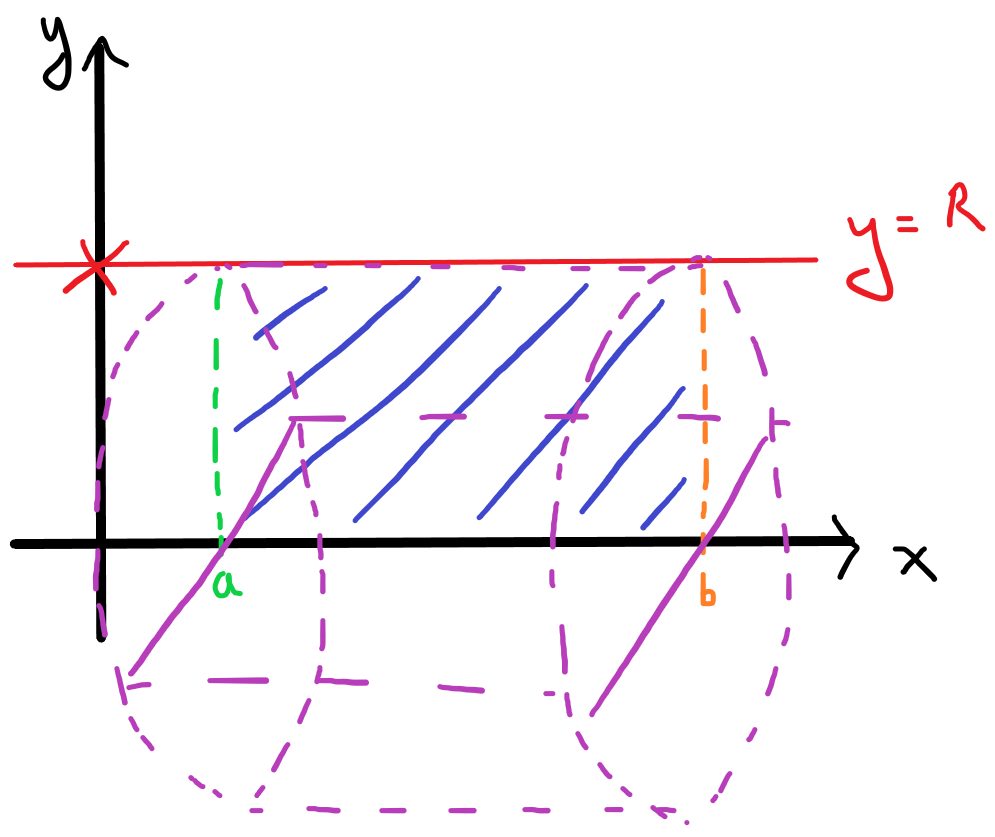
\includegraphics[width=6cm, height=4cm]{assets/ex30-a1-schema.png}
\end{figure}
$$\pi \times \int\limits_a^b (f(x))^2 dx = \pi \times \int\limits_a^b R^2 dx$$ \vspace{0.01cm}

Intéressons-nous à l'intégrale définie \vspace{0.2cm}

\begin{center}
$\displaystyle{\int\limits_a^b R^2 dx = F(b) - F(a)}$ \textit{ssi} $F(x)$ est une primitive de $R^2$ \vspace{0.2cm}

\end{center}

Afin de trouver $F(x)$, il faut résoudre l'intégrale indéfinie \vspace{0.2cm}

$$\int R^2dx = R^2x + c$$ \vspace{0.01cm}

En prenant arbitrairement $F(x)=R^2x$, \vspace{0.2cm}

$$F(b)-F(a) = R^2b-R^2a=R^2\times(b-a)$$ \vspace{0.01cm}

Où $(b-a)$ correspond à la hauteur du cylindre \vspace{0.5cm}

De ce fait,

$$\pi \times \int\limits_a^b R^2 dx = \pi \times R^2 \times h$$

\center{cqfd.}

\newpage
%----------------------------------------------------------------------------------------------------------------------------------------
\flushleft \textbf{a.2) Établir la formule permettant de calculer le volume d'une sphère de rayon \textit{R}}

\begin{figure}[h]
    \textit{\caption{}}\vspace{0.2cm}
    \centering
    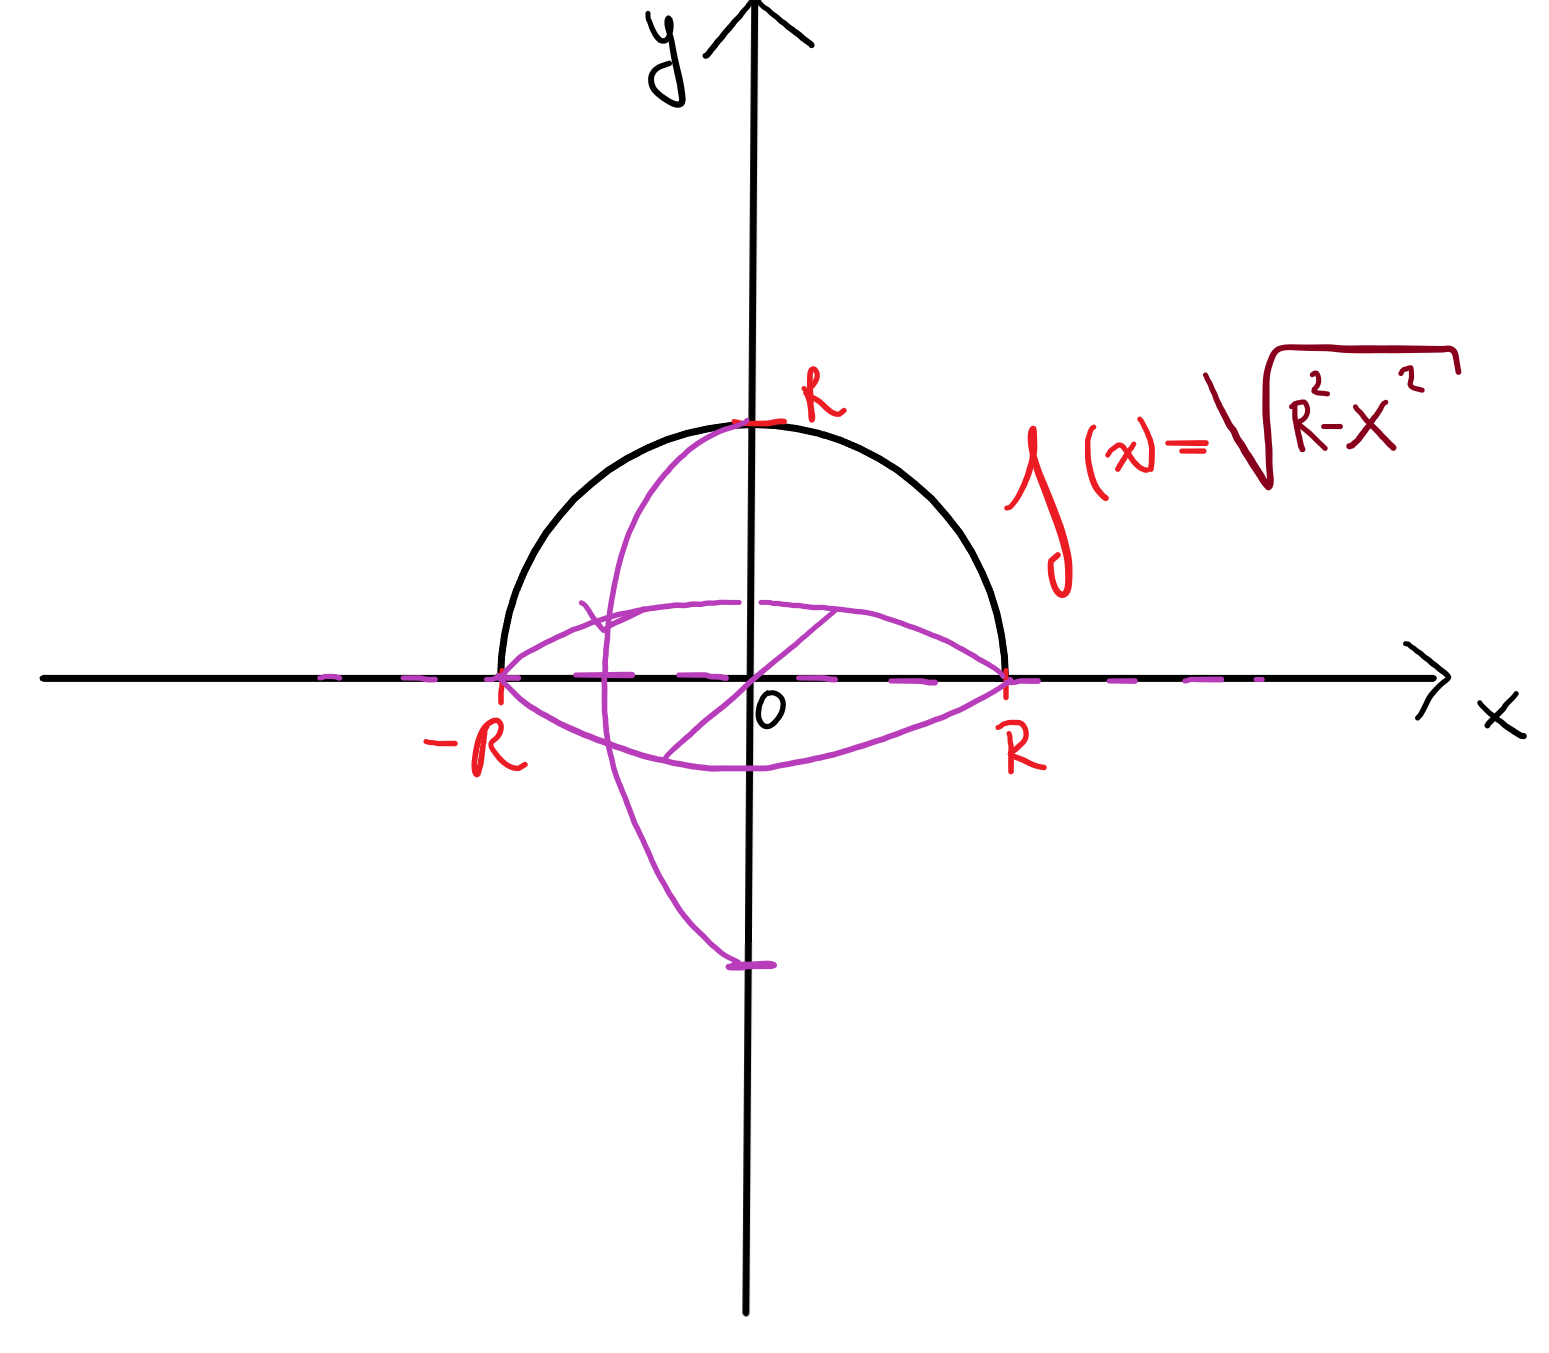
\includegraphics[width=8cm, height=6cm]{assets/ex30-a2-schema.png}
\end{figure}
$$\pi\times\int\limits_a^b(f(x))^2dx = \pi\times\int\limits_{-R}^R\left(\sqrt{R^2-x^2}\right)^2dx=\pi\times\int\limits_{-R}^R({R^2-x^2})dx$$\vspace{0.01cm}

Intéressons-nous à l'intégrale définie\vspace{0.2cm}

\begin{center}
$\displaystyle{\int\limits_{-R}^R({R^2-x^2})dx = F(R) - F(-R)}$ \textit{ssi} $F(x)$ est une primitive de $({R^2-x^2})$\vspace{0.2cm}
\end{center}

Afin de trouver $F(x)$, il faut résoudre l'intégrale indéfinie\vspace{0.2cm}

$$\int(R^2-x^2)dx=R^2x-{x^3\over{3}}+c$$\vspace{0.01cm}

En prenant arbitrairement $F(x)=R^2x-{x^3\over{3}}$,\vspace{0.2cm}

$$F(R)-F(-R)=\left[R^3-{R^3\over{3}}\right]-\left[-R^3+{R^3\over{3}}\right]=2R^3-{2R^3\over{3}}={4R^3\over{3}}$$\vspace{0.01cm}

De ce fait,

$$\pi\times\int\limits_{-R}^R({R^2-x^2})dx = \pi\times{4R^3\over{3}}$$

\center{cqfd.}

\newpage
%----------------------------------------------------------------------------------------------------------------------------------------
\flushleft \textbf{a.3) Établir la formule permettant de calculer le volume d'un cône droit de rayon \textit{R} et de hauteur \textit{h}}

\begin{figure}[h]
    \textit{\caption{}}\vspace{0.2cm}
    \centering
    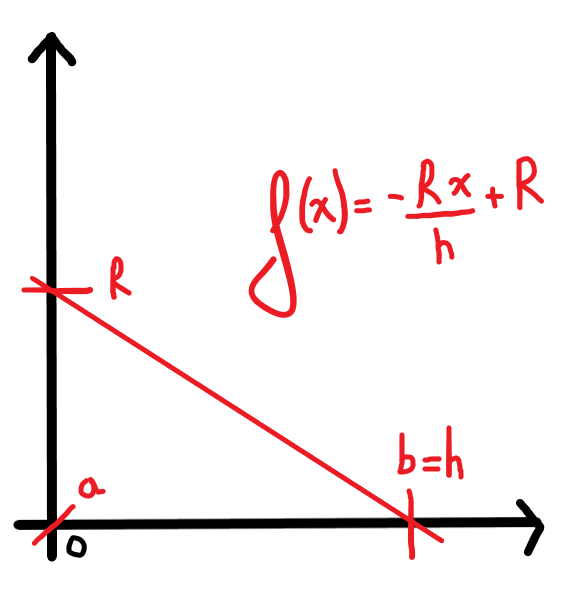
\includegraphics[width=4cm, height=4cm]{assets/ex30-a3-schema.png}
\end{figure}
Trouver la fonction est plus long pour ce cas-ci.
Nous savons que $f(a)=f(0)=R$ et que $f(b)=f(h)=0$\vspace{0.5cm}

La fonction se présente donc sous la forme $\displaystyle{f(x)={y_b-y_a\over{x_b-x_a}}\times{x+R}}$, ce qui revient à $\displaystyle{f(x)={-Rx\over{h}}+R}$\vspace{0.2cm}

$$\pi\times\int\limits_a^b(f(x))^2dx=\pi\times\int\limits_0^h\left({-Rx\over{h}}+R\right)^2dx=\pi\times\int\limits_0^h\left({R^2x^2\over{h^2}}-{2R^2x\over{h}}+R^2\right)dx$$\vspace{0.01cm}

Intéressons-nous à l'intégrale définie\vspace{0.2cm}

\begin{center}
$\displaystyle{\int\limits_0^h\left({R^2x^2\over{h^2}}-{2R^2x\over{h}}+R^2\right)dx = F(h)-F(0})$ \textit{ssi} $F(x)$ est une primitive de $\displaystyle{\left({R^2x^2\over{h^2}}-{2R^2x\over{h}}+R^2\right)}$\vspace{0.01cm}
\end{center}

Afin de trouver $F(x)$, il faut résoudre l'intégrale indéfinie\vspace{0.2cm}

$$\int\left({R^2x^2\over{h^2}}-{2R^2x\over{h}}+R^2\right)dx={R^2x^3\over{3}h^2}-{R^2x^2\over{h}}+R^2x+c$$\vspace{0.01cm}

En choisissant arbitrairement

$$F(x)={R^2x^3\over{3}h^2}-{R^2x^2\over{h}}+R^2x$$\vspace{0.01cm}

Le calcul de l'intégrale définie devient\vspace{0.2cm}

$$F(h)-F(0)={R^2h^3\over{3}h^2}-{R^2h^2\over{h}}+R^2h={R^2h\over{3}}-R^2h+R^2h={R^2h\over{3}}$$\vspace{0.01cm}

De ce fait,

$$\pi\times\int\limits_0^h\left({R^2x^2\over{h^2}}-{2R^2x\over{h}}+R^2\right)dx=\pi\times{R^2h\over{3}}$$

\center{cqfd.}

\newpage
%----------------------------------------------------------------------------------------------------------------------------------------
\flushleft \textbf{b. Quel est le rapport des volumes d'un cône droit et d'un cylindre droit de même rayon et de même hauteur}\vspace{0.5cm}

Le rapport est égal à $$\displaystyle{\pi \times R^2 \times h \over{3}} \times {1\over{\pi \times R^2 \times h}}={1\over{3}}$$

%----------------------------------------------------------------------------------------------------------------------------------------
\flushleft \textbf{c. Comparer le volume d'une sphère de rayon \textit{R} et celui du cylindre qui lui est circonscrit}\vspace{0.5cm}

Le volume d'une sphère de rayon R est de $\pi\times{4R^3\over{3}}$\vspace{0.5cm}

Le cylindre qui lui est circonscrit possède, par définition, le même rayon \textit{R}, qui est égal à sa hauteur \textit{h}.\vspace{0.5cm}

Son volume est donc de $\pi \times R^2 \times h=\pi \times R^3$ \vspace{0.5cm}

Le rapport entre le volume de la sphère et le volume du cylindre qui lui est circonscrit est égal à

$$\displaystyle{\pi\times4R^3\over{3}}\times{1\over{\pi \times R^3}}={4\over{3}}$$

%----------------------------------------------------------------------------------------------------------------------------------------
\flushleft \textbf{d. Un tore est un solide de révolution engendré par un cercle tournant autour d'une droite située dans son plan mais ne passant pas par son centre. Montre que le volume V d'un tore engendré par le mouvement d'un cercle de rayon \textit{R} et dont le centre est situé à une distance $a$ de la droite autour de laquelle il tourne, est donné par $V=2a\pi^2 R^2$.}\vspace{0.5cm}

Pour réaliser cet exercice, nous avons besoin des fonctions $f(x)=\sqrt{R^2-x^2}+a$ et $g(x)=-\sqrt{R^2-x^2}+a$

\begin{figure}[h]
    \textit{\caption{Ici, $a=4$ et $R=2$}}\vspace{0.2cm}
    \centering
    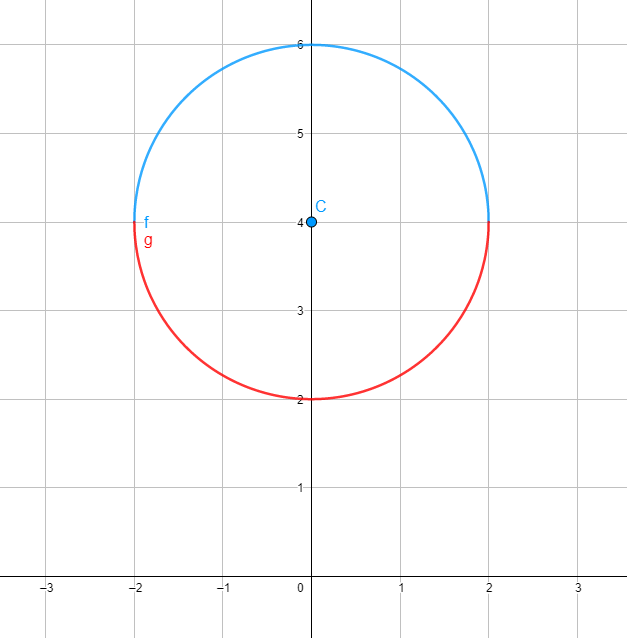
\includegraphics[width=6cm, height=6cm]{assets/ex30-d-schema.png}
\end{figure}


\begin{center}Afin de trouver le volume du tore formé par la révolution de ces deux fonctions, j'ai réalisé le calcul suivant:\end{center}\vspace{0.2cm}

$$\pi\times\int\limits_{-R}^R\left(\sqrt{R^2-x^2}+a\right)^2dx - \pi\times\int\limits_{-R}^R\left(-\sqrt{R^2-x^2}+a\right)^2dx$$

$$=\pi\times\left[\left(\int\limits_{-R}^R \left(a^2+2a\sqrt{R^2-x^2}+R^2-x^2\right)dx\right)-\left(\int\limits_{-R}^R \left(a^2-2a\sqrt{R^2-x^2}+R^2-x^2\right)dx\right)\right]$$

\newpage
%----------------------------------------------------------------------------------------------------------------------------------------
\textbf{1. Recherche des primitives de $f(x)$ et $g(x)$}\vspace{0.5cm}

1.1. Recherche de $F(x)$ \vspace{0.5cm}

\hspace{0.8cm} Passage à l'intégrale indéfinie\vspace{0.2cm}

$$\int (a^2+2a\sqrt{R^2-x^2}+R^2-x^2)dx$$\vspace{0.01cm}

\hspace{0.8cm} Décomposition en somme d'intégrales\vspace{0.2cm}

$$=\int a^2dx + 2a\int(\sqrt{R^2-x^2})dx + \int R^2dx - \int x^2dx$$

$$=a^2x + aR^2\arcsin({x\over{R}}) + ax\sqrt{R^2-x^2} + R^2x - {x^3\over{3}} + c$$

\begin{center}
\hspace{0.8cm} Prenons $\displaystyle{F(x)=a^2x + aR^2\arcsin({x\over{R}}) + ax\sqrt{R^2-x^2} + R^2x - {x^3\over{3}}}$ comme primitive de $f(x)$\vspace{0.2cm}
\end{center}

1.2 Recherche de $G(x)$ \vspace{0.5cm}

\hspace{0.8cm} Passage à l'intégrale indéfinie\vspace{0.2cm}

$$\int (a^2-2a\sqrt{R^2-x^2}+R^2-x^2)dx$$\vspace{0.01cm}

\hspace{0.8cm} Décomposition en somme d'intégrales\vspace{0.2cm}

$$=\int a^2dx - 2a\int(\sqrt{R^2-x^2})dx + \int R^2dx - \int x^2dx$$

$$=a^2x - aR^2\arcsin({x\over{R}}) - ax\sqrt{R^2-x^2} + R^2x - {x^3\over{3}} + c$$

\begin{center}
\hspace{0.8cm} Prenons $\displaystyle{G(x)=a^2x - aR^2\arcsin({x\over{R}}) - ax\sqrt{R^2-x^2} + R^2x - {x^3\over{3}}}$ comme primitive de $g(x)$\vspace{0.2cm}
\end{center}

\textbf{2. Résolution des deux intégrales définies}\vspace{0.5cm}

2.1 Calcul de $F(R)-F(-R)$\vspace{0.2cm}

$$=\left[{2R^3\over{3}}+{aR^2\pi\over{2}}+a^2R\right]-\left[{-2R^3\over{3}}-{aR^2\pi\over{2}} - a^2R\right]$$

$$={4R^3\over{3}}+aR^2\pi + 2a^2R$$\vspace{0.01cm}

2.2. Calcul de $G(R)-G(-R)$\vspace{0.2cm}

$$=\left[{2R^3\over{3}}-{aR^2\pi\over{2}}+a^2R\right]-\left[{-2R^3\over{3}}+{aR^2\pi\over{2}} - a^2R\right]$$

$$={4R^3\over{3}}-aR^2\pi + 2a^2R$$

\newpage
%----------------------------------------------------------------------------------------------------------------------------------------

\textbf{3. Formule finale}\vspace{0.2cm}

$$=\pi\times\left[\left(\int\limits_{-R}^R (a^2+2a\sqrt{R^2-x^2}+R^2-x^2)dx\right)-\left(\int\limits_{-R}^R (a^2-2a\sqrt{R^2-x^2}+R^2-x^2)dx\right)\right]$$

$$=\pi\times\left[\left({4R^3\over{3}}+aR^2\pi + 2a^2R\right)-\left({4R^3\over{3}}-aR^2\pi + 2a^2R\right)\right]$$

$$=\pi\times\left[2aR^2\pi\right]$$

$$=2aR^2\pi^2$$

\center{cqfd.}

\flushleft \textbf{e. Un \textit{segment sphérique} est une portion de sphère coupée par deux plans parallèles. Montrer que le volume $V$ du segment sphérique de largueur h et de rayon $a$ et $b$, engendré par la rotation autour de l'axe $Ox$ de la surface est donné par}
$$\displaystyle{V={\pi h^3\over{6}}+{\pi h(a^2+b^2)\over{2}}}$$
Afin de réaliser cet exercice, j'ai utilisé les sources suivantes:
\begin{center}
mathworld.wolfram.com/SphericalSegment.html et http://ambrsoft.com/TrigoCalc/Sphere/Cap/SphereCap.html
\end{center}
La technique de démonstration diffère de celle qui nous est demandée dans le livre, mais le résultat reste le même. Seules l'orientation de la figure et l'intégrale sont changées et, au lieu de pivoter autour de l'axe $Ox$, la surface pivote autour de l'axe $Oy$.
\begin{figure}[h]
    \textit{\caption{}}\vspace{0.2cm}
    \centering
    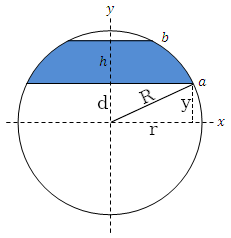
\includegraphics[width=6.5cm, height=6.5cm]{assets/ex30-e-schema.png}
\end{figure}
\begin{center}
Appelons $R$ le rayon de la sphère et $h$ la hauteur du segment. 

Le rayon des cercles supérieur et inférieur sont appelés respectivement $a$ et $b$. 

Appelons $d$ la distance entre le centre de la sphère et le plus grand diamètre du segment. 

Le rayon qui est parallèle au segment est appelé $r$ tandis que la hauteur qui les distingue est appelée $y$.

Nous pouvons déjà poser, grâce au théorème de Pythagore, $r^2 = R^2-y^2$
\end{center}
$$V=\int\limits_d^{d+h} \pi r^2 dy$$
$$=\pi \times \int\limits_d^{d+h} (R^2-y^2)dy$$
$$=\pi \times \left[ R^2 y - {y^3\over{3}}\right]_d^{d+h} $$
$$=\pi \times \left[ \left( R^2(d+h) - {(d+h)^3\over{3}} \right) - \left( R^2d - {d^3\over{3}} \right) \right]$$
$$=\pi \times \left[ R^2h - {1\over{3}} \left( d^3+3d^2h+3dh^2+h^3-d^3 \right) \right]$$
$$=\pi h \times \left( R^2-d^2-hd-{h^2\over{3}} \right)$$\vspace{0.1cm}

Grâce à Pythagore, nous pouvons trouver certaines égalités:

$$a=\sqrt{R^2-d^2}$$
$$b=\sqrt{R^2-(d+h)^2} = \sqrt{R^2-d^2-2dh-h^2}$$
$$d={a^2-b^2-h^2\over{2h}}$$
$$R= \sqrt{{[(a-b)^2+h^2][(a+b)^2+h^2]\over{4h^2}}}$$\vspace{0.1cm}

Remplacer ces paramètres nous donne:

$$V = \pi h \times \left[{1\over{2}}(a^2+b^2+h^2)-{1\over{3}}h^2 \right]$$
$$= \pi h \times \left( {1\over{2}}a^2 + {1\over{2}}b^2 + {1\over{6}}h^2 \right)$$
$$={1\over{6}} \pi h \times (3a^2 + 3b^2 + h^2 )$$
$$={\pi h^3\over{6}} + {\pi h (a^2+b^2)\over{2}}$$

\begin{center}
cqfd.
\end{center}

%----------------------------------------------------------------------------------------------------------------------------------------
\section*{Exercice 42 (p. 161) : château d'eau}\vspace{0.2cm}

\flushleft Le réservoir sphérique d'un château d'eau a un rayon de 6 $m$.\vspace{0.1cm}

a. Calculer, en $m^3$, la capacité maximum de ce réservoir.

$$V = {\pi \times 4R^2\over{3}} = {\pi \times 4.6^2\over{3}} = 904,77 m^3$$\vspace{0.1cm}

b. Calculer, en $m^3$, le volume d'eau contenu dans la partie sphérique de ce réservoir lorsque la hauteur de l'eau y est

\hspace{1cm}1) de 4 $m$ ;

$$V=\pi \times \int\limits_{-6}^{-2} \left( \sqrt{6^2-x^2} \right)^2dx$$
$$=\pi \times \int\limits_{-6}^{-2} (36-x^2)dx$$
$$=\pi \times \left[ 36x-{x^3\over{3}} \right]_{-6}^{-2}$$
$$=\pi \times \frac{224}{3}$$
$$=234,572251 m^3$$

\newpage
%----------------------------------------------------------------------------------------------------------------------------------------

\hspace{1cm}2) de 7 $m$ ;

$$V=\pi \times \int\limits_{-6}^{1} \left( \sqrt{6^2-x^2} \right)^2dx$$
$$=\pi \times \int\limits_{-6}^{1} (36-x^2)dx$$
$$=\pi \times \left[ 36x-{x^3\over{3}} \right]_{-6}^{1}$$
$$=\pi \times \frac{539}{3}$$
$$=564,4394801 m^3$$

\hspace{1cm}3) de $x$ $m$ ($0 \leq x \leq 12$).

$$V=\pi \times \int\limits_{-6}^{x-6} \left( \sqrt{6^2-x^2} \right)^2dx$$
$$=\pi \times \int\limits_{-6}^{x-6} (36-x^2)dx$$
$$=\pi \times \left[ 36x-{x^3\over{3}} \right]_{-6}^{x-6}$$
$$=\pi \times \left( -\frac{(x-6)^3}{3}+36x-72 \right)$$

\begin{figure}[h]
    \textit{\caption{$f(x)=\sqrt{36-x^2}$}}\vspace{1cm}
    \centering
    \includegraphics[width=16cm, height=10cm]{assets/ex42-schema.png}
\end{figure}

\newpage
%----------------------------------------------------------------------------------------------------------------------------------------
\section*{Exercice 16 (p. 232) : l'échelle}\vspace{0.2cm}

\begin{flushleft}
a. Une échelle longue de 10 mètres est appuyée contre un mur et glisse sur le sol : le pied de l'échelle s'éloigne

\hspace{13pt}du pied du mur et son sommet descend le long du mur jusqu'à ce que l'échelle soit couchée sur le sol.\vspace{0.1cm}

\hspace{13pt}Détermine la trajectoire du point $M$ situé au milieu de l'échelle lorsque celle-ci passe de la position verticale

\hspace{13pt}à la position horizontale.
\end{flushleft}

\begin{figure}[h]
    \textit{\caption{La trajectoire du point $M$ est un arc de cercle de centre d'équation $C \equiv x^2+y^2=5$}}\vspace{0.2cm}
    \centering
    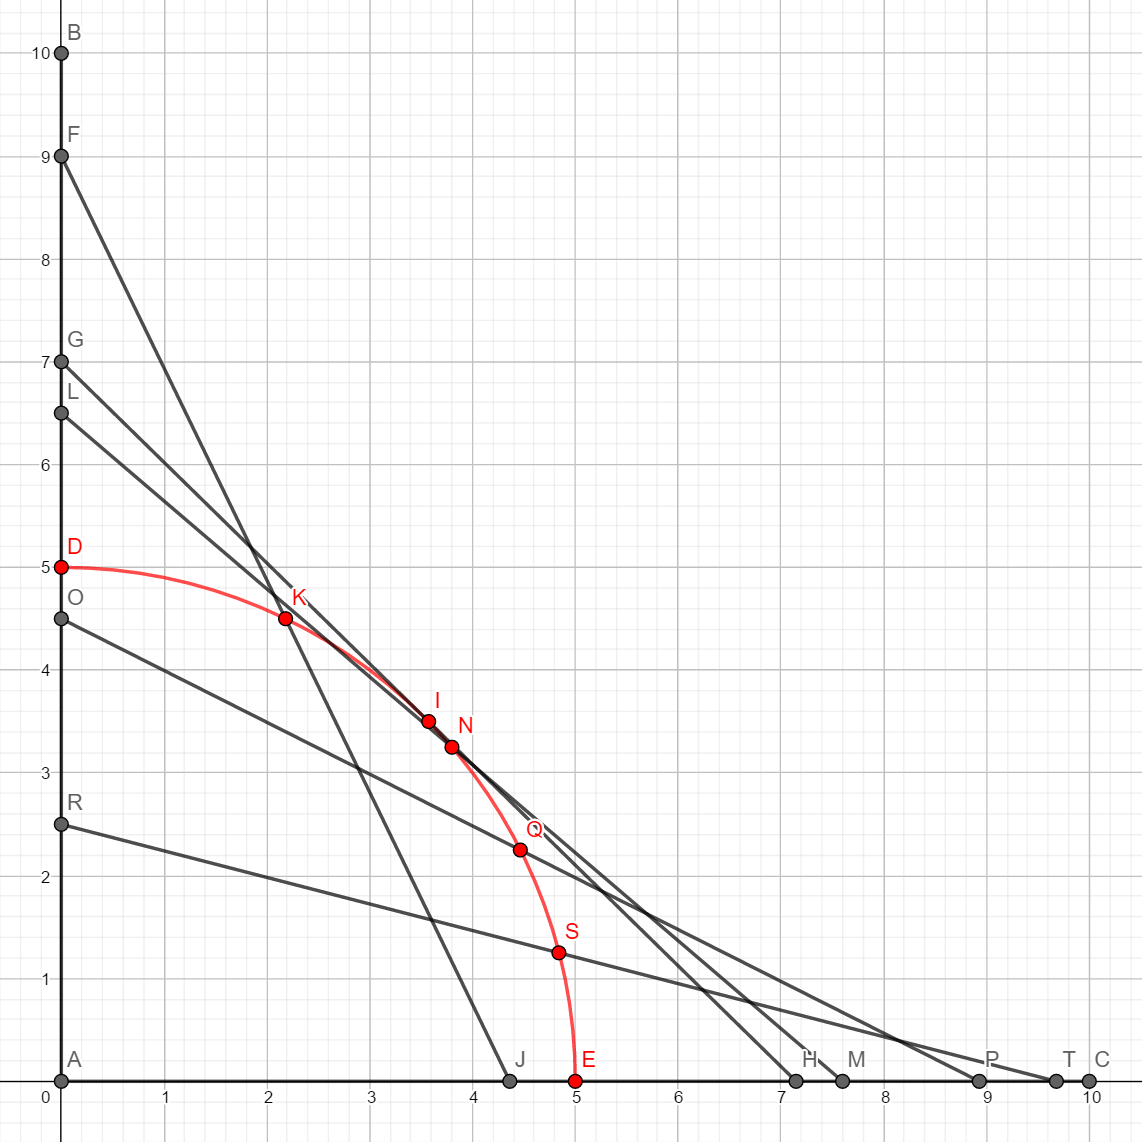
\includegraphics[width=7.5cm, height=7.5cm]{assets/ex16-a-schema.png}
\end{figure}

%----------------------------------------------------------------------------------------------------------------------------------------
\begin{flushleft}
b. Dans la même situation, déterminer la trajectoire du point $P$ situé au quart de l'échelle à partir du sommet

\hspace{13pt}lorsque celle-ci passe de la position verticale à la position horizontale.
\end{flushleft}

\begin{figure}[h]
    \textit{\caption{La trajectoire du point $P$ se trouve sur une ellipse d'équation $E_P \equiv 900x^2+100y^2=5624$}}\vspace{0.2cm}
    \centering
    \includegraphics[width=7.5cm, height=7.5cm]{assets/ex16-b-schema.png}
\end{figure}
\newpage
%----------------------------------------------------------------------------------------------------------------------------------------
\begin{flushleft}
c. Même question avec le point $Q$ situé au quart de l'échelle à partir du pied.\vspace{0.1cm}
\end{flushleft}

\begin{figure}[h]
    \textit{\caption{La trajectoire du point $Q$ se trouve sur une ellipse d'équation $E_Q \equiv 100x^2+900y^2=5624$}}\vspace{0.2cm}
    \centering
    \includegraphics[width=7.5cm, height=7.5cm]{assets/ex16-c-schema.png}
\end{figure}

\vspace{12.5cm}

\begin{center}
\vspace{1cm}Ce travail a été réalisé en \LaTeX . \vspace{0.2cm}

Les figures 4, 6, 7, 8 et 9 ont été construites sur \textit{GeoGebra}.\vspace{0.2cm}

Code source disponible sur \textit{GitHub} à cette adresse : https://github.com/noehov/coursmath6
\end{center}

\end{document}
